% \chapter{\ifproject%
% \ifenglish Experimentation and Results\else การทดลองและผลลัพธ์\fi
% \else%
% \ifenglish System Evaluation\else การประเมินระบบ\fi
% \fi}
\chapter{
    \ifenglish Experimentation and Results\else การทดลองและผลลัพธ์\fi
}

\definecolor{eyrie}{HTML}{1E90FF}
\definecolor{marquise}{HTML}{FF6400}

% ในบทนี้จะทดสอบเกี่ยวกับการทำงานในฟังก์ชันหลักๆ

\section{Experiment Setup}

\subsection{Introductory Experiment}
For the introductory experiment, we will use random decision agent as it has the most basic implementation. Since we have not implemented \RootAI, we will conduct experiments by simulating \RootOurs \ with random actions option turned on, and collect the results. 

We will run 100,000 \glspl{playout} using a random decision agent as each faction and collect the following statistics:
\begin{itemize}
    \item winning faction: \Marquise{} / \Eyrie
    \item winning condition: 30 victory points (vp)
    \item number of turns played (the number of birdsong phase played)
    \item whose turn was it when the game ends: \Marquise{} / \Eyrie
    \item victory points of \Marquise{} when the game ends
    \item victory points of \Eyrie{} when the game ends
\end{itemize}

\subsection{Main Experiment}
The main experiment consists of 2 phases. We will make multiple variants of MCTS and have them play against a ``base'' agent. 

\subsubsection{Setup} \label{main-exp-setup}
The base agent is an MCTS agent. It was used to play against the Random agent. The results shows that both \Marquise{} and \Eyrie{}, with base agent are able to consistently win most of the rounds against the Random agent. This means that we cannot use the Random agent as base since all MCTS agents would likely have very high win rate.

The base agent's MCTS parameters are as follows:
\begin{enumerate}
    \item \textbf{\texttt{reward-function}}: \texttt{vp-difference}
    \item \textbf{\texttt{expand-count}}: 100
    \item \textbf{\texttt{rollout-no}}: 1
    \item \textbf{\texttt{time-limit}}: -1
    \item \textbf{\texttt{action-count-limit}}: 20
    \item \textbf{\texttt{best-action-policy}}: \texttt{robust}
\end{enumerate}

The main experiment's MCTS variants are permutations of these parameters:
\begin{enumerate}
    \item \textbf{\texttt{reward-function}}: \texttt{win}, \texttt{vp-difference}, \texttt{vp-difference-relu} (\texttt{vp-difference-bin} is excluded because it is the same as \texttt{vp-difference-relu} but is unable to separate a ``very good'' rollout from a ``good'' rollout.)
    \item \textbf{\texttt{expand-count}}: 50, 100, 200
    \item \textbf{\texttt{rollout-no}}: 1 (fixed to 1 because we have, in a way, eliminated nondeterminism in our simulation)
    \item \textbf{\texttt{time-limit}}: -1 (means no time limit. because the rollout time are so fast that the time limit is ignorable)
    \item \textbf{\texttt{action-count-limit}}: 20, 100, 200, -1 (-1 means no limit)
    \item \textbf{\texttt{best-action-policy}}: \texttt{max}, \texttt{robust}, \texttt{secure}
    % TODO: why is UCB removed?
    % TODO: recheck the reasons for these param choices
\end{enumerate}
These parameters resulted in 108 variants for each faction.

\subsubsection{Phase 1}
For the first phase, as there are 108 MCTS variants and 2 factions, there will be 216 battles in this phase. Each battle will be run for 100 rounds to minimize random deviation.

\subsubsection{Phase 2}
For the second phase, the top variants from the first phase will be selected to continue in this phase. The metrics of selection is ``win rate'' against the base variant. Unless some variant achieved 100\% win rate (win all 100 rounds), it is unlikely that the variants will have overlapping win rates, though if that were to be the case, other metrics will be used such as ``average turns to win'', etc. The top 5 variants for each faction will be selected. Then they all play against each of the other faction's, i.e., a ``Team Round-Robin''. There will be 25 battles in this phase. Each battle will be run for 1000 rounds.

\subsubsection{Final}
Finally, the best performing variant from each faction will be selected to be the ``best MCTS variant'' for that faction.



\section{Results}

\subsection{Introductory Experiment's Results}

% \begin{figure}
%     \centering
%     \begin{tikzpicture}
%         \begin{axis}[
%             width  = 0.5*\textwidth,
%             height = 8cm,
%             major x tick style = transparent,
%             ybar=2*\pgflinewidth,
%             bar width=24pt,
%             ymajorgrids = true,
%             ylabel = {Number of Wins},
%             symbolic x coords={Dominance Card,Victory Point},
%             xtick = data,
%             enlarge x limits=0.5,
%             enlarge y limits=0.1,
%             ymax = 1000,
%             legend cell align=left,
%             legend style={
%                 at={(0.5,-0.15)},
%                 anchor=north,
%                 legend columns=-1
%             },
%             nodes near coords,
%         ]
%             \addplot[style={eyrie,fill=eyrie,mark=none}]
%                 coordinates {(Dominance Card, 230) (Victory Point,44)};
    
%             \addplot[style={marquise,fill=marquise,mark=none}]
%                  coordinates {(Dominance Card,695) (Victory Point,31)};
    
%             \legend{\Eyrie, \Marquise}
%         \end{axis}
%     \end{tikzpicture}
%     \caption{The number of wins grouped by winning condition}
%     \label{fig:wins-by-winner-condition}
% \end{figure}

\begin{figure}
    \begin{center}
      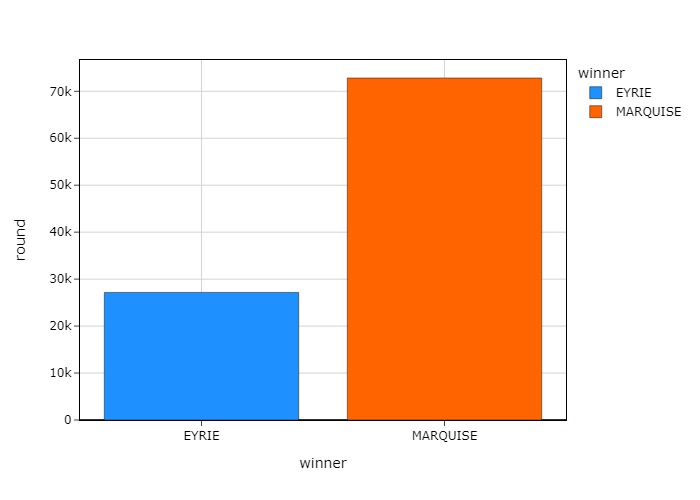
\includegraphics[width=\textwidth]{./images/fig-random-random-win.jpeg}
    \end{center}
    \caption{The number of wins}
    \label{fig:wins}
  \end{figure}

% \subsubsection{High dominance card wins} \label{high-dominance-card-wins}
% Dominance card wins happen way more often than victory points wins as seen in Figure \ref{fig:wins}. Our speculation is that it is the action generation in \RootOurs{} that makes the ``Activate Dominance Card'' action have a higher likelihood of being picked. \RootOurs{} generates actions in a manner that is more suitable for human players, e.g., in the move action, the agent needs to select a start clearing, then a destination clearing, and then how many warriors to move. These are done as three separate actions, while in reality, the action of ``Move X warriors from A to B'' should be counted as one action.

% \subsubsection{\Marquise's high dominance card wins}
% \Marquise \ have a higher chance to win with dominance card as seen in Figure \ref{fig:wins}. Our speculation is that because at the start of the round, \Marquise{} have control over clearings except the one that \Eyrie{} starts in, therefore, if \Eyrie{} does not play properly to take control of the clearings, \Marquise{} will likely win upon the activation of a dominance card of any suit.

% Additionally, games with \Marquise's dominance card wins take fewer turns, as seen in Figure \ref{fig:turns-to-dominance-win}. Which should be due to \Marquise \ starting with more clearings under control.

\subsubsection{\Marquise's high victory points wins}

% \Eyrie \ have a higher chance to win with victory points as seen in Figure \ref{fig:wins}. Although there are not many data for rounds with victory points wins, our experience during development where we turned of the dominance card mechanics also have more \Eyrie \ victory points win. Our speculation is that this is due to \Eyrie's passive earning of victory points, all they need to do is protect their roosts and don't turmoil too much. In contrast, \Marquise \ needs to actively build buildings to earn victory points, which from the issue about action generation in Section \ref{high-dominance-card-wins}, action of building buildings might not have the correct likelihood of being picked.

% Additionally, games with \Eyrie's victory points wins take more turns than those with \Marquise's, as seen in Figure \ref{fig:turns-to-vp-win}. Which should be due to \Eyrie \ having passive, continuous earning of victory points every turn while \Marquise's earnings is more like a burst of victory points every time they build a building.



% \begin{figure}
%     \centering
%     \begin{tikzpicture}
%         \begin{axis}[
%             ytick={1,2},
%             yticklabels={\Eyrie, \Marquise},
%             xlabel={Number of Turns},
%             ylabel={Faction},
%             boxplot/draw direction=x,
%         ]
%             \addplot+[
%                 boxplot prepared={
%                     median=42, 
%                     upper quartile=59.5, 
%                     lower quartile=30, 
%                     upper whisker=304, 
%                     lower whisker=14
%                 }, eyrie, draw=eyrie
%             ] coordinates {};

%             \addplot+[
%                 boxplot prepared={
%                     median=27.0, 
%                     upper quartile=47.0, 
%                     lower quartile=19.0, 
%                     upper whisker=339.0, 
%                     lower whisker=7.0
%                 }, marquise, draw=marquise
%             ] coordinates {};
%         \end{axis}
%     \end{tikzpicture}
%     \caption{Number of turns to achieve a dominance win}
%     \label{fig:turns-to-dominance-win}
% \end{figure}

% \begin{figure}
%     \centering
%     \begin{tikzpicture}
%         \begin{axis}[
%             ytick={1,2,3,4},
%             yticklabels={\Eyrie, \Marquise},
%             xlabel={Number of Turns},
%             ylabel={Faction},
%             boxplot/draw direction=x,
%         ]
%             \addplot+[
%                 boxplot prepared={
%                     median=33, 
%                     upper quartile=42, 
%                     lower quartile=26, 
%                     upper whisker=58, 
%                     lower whisker=18
%                 }, eyrie, draw=eyrie
%             ] coordinates {};

%             \addplot+[
%                 boxplot prepared={
%                     median=25.0, 
%                     upper quartile=27.0, 
%                     lower quartile=22.5, 
%                     upper whisker=37.0, 
%                     lower whisker=17.0
%                 }, marquise, draw=marquise
%             ] coordinates {};
%         \end{axis}
%     \end{tikzpicture}
%     \caption{Number of turns to achieve a victory points win}
%     \label{fig:turns-to-vp-win}
% \end{figure}

\subsection{Main Experiment's Result}

\subsubsection{Phase 1}

% \textbf{Top 5 Variants}

In this section, parameters \texttt{rollout-no} and \texttt{time-limit} are not displayed in the tables as they are fixed to 1 and -1 (no-limit), respectively.

The results of top 5 MCTS variants for \Marquise{} and \Eyrie{} versus the base variant are displayed in Table \ref{tab:mar-top5} and \ref{tab:ey-top5}

\begin{table}%[h!]
    \caption{\Marquise{}'s top 5 MCTS variants versus the base variant}
    \label{tab:mar-top5}
    \centering
    \begin{tabular}{| c || P{1.2cm} | P{1.2cm} || P{4cm} | P{1.2cm} | P{1.2cm} | P{1.2cm} |} 
        \hline
        \bf config no. & \bf  win rate & \bf average match length & \bf reward function & \bf expand count & \bf action count limit & \bf best action policy \\ [0.5ex] \hline 
        86 & 0.61 & 16.787 & \texttt{vp-difference} & 200 & 100 & secure \\ \hline 
        76 & 0.55 & 15.418 & \texttt{vp-difference} & 200 & 20 & robust \\ \hline 
        85 & 0.53 & 15.547 & \texttt{vp-difference} & 200 & 100 & max \\ \hline 
        87 & 0.53 & 16.245 & \texttt{vp-difference-relu} & 200 & 100 & max \\ \hline 
        89 & 0.52 & 15.327 & \texttt{vp-difference-relu} & 200 & 100 & secure \\ \hline %[1ex] 
        \hline
    \end{tabular}
\end{table}

\begin{table}%[h!]
    \caption{\Eyrie{}'s top 5 MCTS variants versus the base variant}
    \label{tab:ey-top5}
    \centering
    \begin{tabular}{| c || P{1.2cm} | P{1.2cm} || P{4cm} | P{1.2cm} | P{1.2cm} | P{1.2cm} |} 
        \hline
        \bf config no. & \bf  win rate & \bf average match length & \bf reward function & \bf expand count & \bf action count limit & \bf best action policy \\ [0.5ex] \hline 
        184 & 0.81 & 14.519 & \texttt{vp-difference} & 200 & 20 & robust \\ \hline 
        203 & 0.72 & 15.722 & \texttt{vp-difference} & 200 & 200 & secure \\ \hline 
        194 & 0.71 & 15.690 & \texttt{vp-difference} & 200 & 100 & secure \\ \hline 
        212 & 0.71 & 16.676 & \texttt{vp-difference} & 200 & -1 & secure \\ \hline 
        202 & 0.71 & 16.803 & \texttt{vp-difference} & 200 & 200 & robust \\ \hline %[1ex] 
        \hline
    \end{tabular}
\end{table}

% \textbf{Observation: Imbalance in Potential}

\Marquise{}'s win rate ranges from 0.52 to 0.61, while \Eyrie's ranges from 0.71 to 0.81. We speculated that this was due to the difference in ``potential'' between the two factions. \Marquise{}'s playstyle is straight forward because of the fixed action count per turn, while \Eyrie{} has the Decree, which dictates what actions the \Eyrie{} player can perform. The Decree, when built and followed properly, can grant the \Eyrie{} player over twice the action count per turn when compared to \Marquise{}, which grants more potential to earn VPs.

% \textbf{Observation: Impact of each parameters}
Speculation on the impact of each parameters:
\begin{itemize}
    \item Most variant has \texttt{vp-difference}-based reward function. We speculated that this is due to the \texttt{win} option only working if the simulation step reaches a game-ending state.
    \item Every variant has expand count of 200. We speculated that if the MCTS is able to look forward further into the future and see more possible outcomes, it can then select better paths.
    \item The action count limit of 100 is the majority for \Marquise{} while \Eyrie{} has a varying action count limit. We speculated that the action count limit does not necessarily need to be high, but it needs to be at the right value that represents the outcome of a series of actions from the root state. This is because if we look too far into the simulation, the outcomes might not represent our series of actions well, and if we look too close, the outcomes will only represent short-term rewards.
    \item The best action policy also varies between variants. We speculated that each option for this parameter in itself does not impact much, but if combined with fitting options for other parameters, it can then shine.
\end{itemize}






\subsubsection{Phase 2}

% \textbf{Top 1 Variants}

In this section, parameters \texttt{rollout-no} and \texttt{time-limit} are not displayed in the tables as they are fixed to 1 and -1 (no-limit), respectively.

The results of top 5 MCTS variants for \Marquise{} and \Eyrie{} versus the other faction's top 5 MCTS variants are displayed in Table \ref{tab:mar-team-rr} and \ref{tab:ey-team-rr}. The variant with highest win rate in each faction is highlighted in bold.

\begin{table}%[h!]
    \caption{\Marquise{}'s top 5 MCTS variants versus \Eyrie{}'s top 5 MCTS variants}
    \label{tab:mar-team-rr}
    \centering
    \begin{tabular}{| c || P{1.2cm} | P{1.2cm} || P{4cm} | P{1.2cm} | P{1.2cm} | P{1.2cm} |} 
        \hline
        \bf config no. & \bf  win rate & \bf average match length & \bf reward function & \bf expand count & \bf action count limit & \bf best action policy \\ [0.5ex] \hline 
        86 & 0.532 & 15.363 & \texttt{vp-difference} & 200 & 100 & secure \\ \hline 
        76 & 0.390 & 15.727 & \texttt{vp-difference} & 200 & 20 & robust \\ \hline 
        \bf 85 & \bf 0.560 & \bf 15.389 & \bf \texttt{vp-difference} & \bf 200 & \bf 100 & \bf max \\ \hline 
        87 & 0.422 & 15.250 & \texttt{vp-difference-relu} & 200 & 100 & max \\ \hline 
        89 & 0.374 & 15.230 & \texttt{vp-difference-relu} & 200 & 100 & secure \\ \hline %[1ex] 
        \hline
    \end{tabular}
\end{table}

\begin{table}%[h!]
    \caption{\Eyrie{}'s top 5 MCTS variants versus \Marquise{}'s top 5 MCTS variants}
    \label{tab:ey-team-rr}
    \centering
    \begin{tabular}{| c || P{1.2cm} | P{1.2cm} || P{4cm} | P{1.2cm} | P{1.2cm} | P{1.2cm} |} 
        \hline
        \bf config no. & \bf  win rate & \bf average match length & \bf reward function & \bf expand count & \bf action count limit & \bf best action policy \\ [0.5ex] \hline 
        \bf 184 & \bf 0.634 & \bf 13.681 & \bf \texttt{vp-difference} & \bf 200 & \bf 20 & \bf robust \\ \hline 
        203 & 0.520 & 15.388 & \texttt{vp-difference} & 200 & 200 & secure \\ \hline 
        194 & 0.580 & 15.217 & \texttt{vp-difference} & 200 & 100 & secure \\ \hline 
        212 & 0.450 & 15.735 & \texttt{vp-difference} & 200 & -1 & secure \\ \hline 
        202 & 0.538 & 15.517 & \texttt{vp-difference} & 200 & 200 & robust \\ \hline %[1ex] 
        \hline
    \end{tabular}
\end{table}

The variant with the highest win rate versus the other faction's top 5 MCTS variants for \Marquise{} is config number 85 with 0.560 win rate and 15.389 average match length. \Eyrie{}'s is config number 184 with 0.634 win rate and 13.681 average match length. 

% \begin{figure}
%     \centering
%     \begin{tikzpicture}
%         \begin{axis}[
%             ytick={1,2,3,4},
%             yticklabels={\Eyrie, \Marquise},
%             xlabel={Victory Points},
%             ylabel={Faction},
%             boxplot/draw direction=x,
%         ]
%             \addplot+[
%                 boxplot prepared={
%                     median=30.0, 
%                     upper quartile=31.0, 
%                     lower quartile=30.0	, 
%                     upper whisker=33, 
%                     lower whisker=30
%                 }, eyrie, draw=eyrie
%             ] coordinates {};

%             \addplot+[
%                 boxplot prepared={
%                     median=13.0, 
%                     upper quartile=15.25, 
%                     lower quartile=11.0	, 
%                     upper whisker=27, 
%                     lower whisker=9
%                 }, marquise, draw=marquise
%             ] coordinates {};
%         \end{axis}
%     \end{tikzpicture}
%     \caption{Number of Victory Points when \Eyrie{} wins}
% \end{figure}

% \begin{figure}
%     \centering
%     \begin{tikzpicture}
%         \begin{axis}[
%             ytick={1,2,3,4},
%             yticklabels={\Eyrie, \Marquise},
%             xlabel={Victory Points},
%             ylabel={Faction},
%             boxplot/draw direction=x,
%         ]
%             \addplot+[
%                 boxplot prepared={
%                     median=6.0, 
%                     upper quartile=11.0, 
%                     lower quartile=4.0, 
%                     upper whisker=21, 
%                     lower whisker=2
%                 }, eyrie, draw=eyrie
%             ] coordinates {};

%             \addplot+[
%                 boxplot prepared={
%                     median=30.0, 
%                     upper quartile=32, 
%                     lower quartile=30.0	, 
%                     upper whisker=33, 
%                     lower whisker=30
%                 }, marquise, draw=marquise
%             ] coordinates {};
%         \end{axis}
%     \end{tikzpicture}
%     \caption{Number of Victory Points when \Marquise{} wins by victory points condition}
% \end{figure}

% TODO: add result graph